\section{Datenpipeline}
Als Konzeptnachweis ist ein neurales Netzwerk erstellt worden, welches die Nodes und Base-Nodes in den Abbildungen \ref{fig:os} und \ref{fig:xs} von Bildern unterscheiden kann, in denen eben keine Node enthalten ist. 

Dieses wird dann in ein \name{Fully Convolutional Neural Network}\cite{Long2014} umgewandelt, um diese Überprüfung auf einem Bild zusätzlich lokalisieren zu können.

Ein weiteres neurales Netzwerk wird nun erstellt, um die \name{Constraints} zu erkennen.
Hierfür wurden die Symbole, wie sie in den Abbildungen \ref{fig:rs} und \ref{fig:ts} zu sehen sind, benutzt, um Trainingsdaten zu generieren, die wiederum genutzt werden können, um das neurale Netzwerk zu trainieren.
Hierfür wurden die vorher genutzten Nodes zufällig auf einem Bild verteilt und daraufhin zufällig durch Constraints verbunden.

\begin{figure}
  \centering
    \begin{subfigure}[b]{0.3\textwidth}
        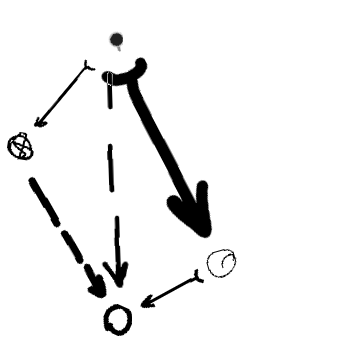
\includegraphics[width=\textwidth]{images/pre_crop.png}
        \caption{}
        \label{fig:pre_crop}
    \end{subfigure}
    \begin{subfigure}[b]{0.3\textwidth}
      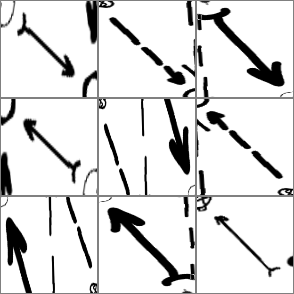
\includegraphics[width=\textwidth]{images/crops.png}
      \caption{}
      \label{fig:crop}
    \end{subfigure}
    \caption{Aus dem links zufällig generiertem Bild wurden die Bilder rechts generiert. Anzumerken ist, dass nur die Bilder der ersten Reihe als korrekt bezeichnet werden.}
    \label{fig:constraint_data}
\end{figure}

Die daraus entstandenen Schnitte werden verformt, um einheitliche Ma{\ss}e zu erhalten.
Des Weiteren werden die Bilder so gespiegelt, dass die erste Node stets oben links im Bild ist.
So sind Bilder nur als korrekt anzusehen, wenn die Verbindung von oben links nach unten rechts dargestellt wird.
Das ist notwendig, um neben der Kategorisierung auch die Richtung der Verbindung zu bestimmen.

Aufbauend auf diesen Algorithmen kann nun eine Datenpipeline programmiert werden, welche anhand eines Bildes zunächst die Nodes erkennt und daraufhin die Bildausschnitte generiert, welche dahingehend untersucht werden können, ob zwischen zwei Nodes eine Constraint existiert.

Die daraus gewonnene Information kann dann in das von \name{mec-2} genutzte JSON Format überführt und der Mechanismus dargestellt werden.
Ein vollständig definierter Mechanismus (alle Gelenke und Glieder, die Anzahl der Freiheitsgrade etc. seien dadurch bekannt) lässt sich so direkt der entsprechenden kinematischen Kette zuordnen.
